\subsection{Objective}
The purpose of this application is to provide an intuitive as well as interactive tool to visualise transformations and their respective effect on the relation to fixed points in three-dimensional space. 

This tool is supposed to support the development of better test cases as well as aid students in the understanding of trigonometry. This tool is mainly aimed at software testers, as it helps them to get a more tangible vision of possible szenarios and now imaginable edge-cases. A secondary target group are (engineering-)students struggeling to get their head around trigonometry.

Since rotations in space become far more difficult to envision if we are concerned about an arbitrary point on the plane, and its relation to fixed points in space, instead of its center, this issue is being addressed by this application.

Although there are many other rotation visualisation tools out there, none of them visualize the relation to fixed points in space, let you move said points or the plane in space and don’t address afroementioned issues.

\newpage
\subsection{Requirements Refinement}
Previous rough user stories now get a clear testable statement assigned to them. 

Requirements that are tagged with \tcbox[colframe=TAGred, colback=TAGred]{\textbf{\footnotesize \acs{M2FR}}}, could not be implemented in time for the planned release and had to be moved to a future release. \newline Since these requirements are not essential for the core functionality and a timely release is ranked higher than the fulfillment of optional requirements, this was considered justified.


\subsubsection{Functional}

    \bgroup
    \def\arraystretch{1.5}
    \setlength\arrayrulewidth{1.2pt}
    \color{textgray}
    \begin{xltabular}{\textwidth}{|X|X|M{1.8cm}|M{1.4cm}|M{1.3cm}|}

\caption*{} \label{tab:Requirements - Functional} \\

\arrayrulecolor{linegray}\hline \rowcolor{lightgray} \multicolumn{1}{|c|}{\color{default}\textbf{Requirement}} & \multicolumn{1}{c|}{\color{default}\textbf{User Story}} & \multicolumn{1}{c|}{\color{default}\textbf{Importance}} & \multicolumn{1}{c|}{\color{default}\textbf{Jira Issue}} & \multicolumn{1}{c|}{\color{default}\textbf{Status}}\\ \hline

 \endfirsthead 
 \multicolumn{5}{c}%
{\tablename\ \thetable{} -- continued from previous page} \\ \hline \multicolumn{1}{|c|}{\textbf{Requirement}} & \multicolumn{1}{c|}{\textbf{User Story}} & \multicolumn{1}{c|}{\textbf{Importance}} & \multicolumn{1}{c|}{\textbf{Jira Issue}} & \multicolumn{1}{c|}{\textbf{Status}}\\ \hline 
\endhead \hline 
\multicolumn{5}{|r|}{{Continued on next page}} \\ \hline 
\endfoot

\hline 
 \endlastfoot 
\textbf{1.} A maximum of 5 bird Avatar-elements shall be displayed in the main page. The most recent bird shall be at the front of the list. \newline \textbf{2.} An Indicator shall signal if more than 5 birds were added. & As a user I want to see an overview of my added birds in the main page & \tcbox[colframe=TAGred, colback=TAGred]{\textbf{\footnotesize HIGH}} & {\color{purpleT}\ttfamily DLMCSPSE-224} & \tcbox[colframe=TAGgreen, colback=TAGgreen]{\textbf{\footnotesize DONE}} \\ \hline 
  \textbf{1.} Birds shall be addable by providing the initial XYZ-coordinates. If no coordinate or a NaN-Value is provided, it shall be interpreted as 0. \newline \textbf{2.} A bird shall not be addable if its distance is greater than 100m from the plane. If such values are provided, the user shall be informed via a Toast-Message. \newline \textbf{3.} A bird shall be removable via a simple click on an X-icon, coloured in the birds highlight colour, on/adjacent to the bird’s avatar. & As a user I want to easily add and remove nearby threats without leaving the main page & \tcbox[colframe=TAGred, colback=TAGred]{\textbf{\footnotesize HIGH}} & {\color{purpleT}\ttfamily DLMCSPSE-225} & \tcbox[colframe=TAGgreen, colback=TAGgreen]{\textbf{\footnotesize DONE}} \\ \hline 
  \textbf{1.} A click on the birds avatar shall select the corresponding bird. \newline \textbf{2.} The fact that a bird is selected shall be visible in the UI. \newline \textbf{3.} Only one bird shall be selectable at a time. \newline \textbf{4.} A second click on a selected bird shall deselect said bird. \newline & As a user I want to be able to highlight a specific bird to make this specific bird stand out in the UI. & \tcbox[colframe=TAGred, colback=TAGred]{\textbf{\footnotesize HIGH}} & {\color{purpleT}\ttfamily DLMCSPSE-226} & \tcbox[colframe=TAGgreen, colback=TAGgreen]{\textbf{\footnotesize DONE}} \\ \hline 
  \textbf{1.} The user shall be able to translate the plane in space by adding values to the current position of the planes XYZ-axis. \newline \newline \textbf{2.} If no coordinate or a NaN-Value is provided, it shall be interpreted as 0. \newline \newline \textbf{3.} The plane shall not be able to be translated below ground. \newline \textbf{a.}  If this would be the case, the plane shall not be moved and an error shall be displayed. & As a user I want to move the plane in space. & \tcbox[colframe=TAGred, colback=TAGred]{\textbf{\footnotesize HIGH}} & {\color{purpleT}\ttfamily DLMCSPSE-228} & \tcbox[colframe=TAGgreen, colback=TAGgreen]{\textbf{\footnotesize DONE}} \\ \hline 
  \textbf{1.} The plane shall not be distorted → the viewport shall remain a cube. \newline\newline \textbf{2.} The view shall always be centred around the plane. \newline\newline \textbf{3.} The side length of aforementioned cube shall be the distance to the furthest threat and at least 10. & As a user I always want to see the plane centred and as close as possible. & \tcbox[colframe=TAGred, colback=TAGred]{\textbf{\footnotesize HIGH}} & {\color{purpleT}\ttfamily DLMCSPSE-229} & \tcbox[colframe=TAGgreen, colback=TAGgreen]{\textbf{\footnotesize DONE}} \\ \hline 
  All birds shall be displayed as a point in space in the colour of the corresponding bird. & As a user I want to see my added birds in the 3D-Diagram in the main page & \tcbox[colframe=TAGred, colback=TAGred]{\textbf{\footnotesize HIGH}} & {\color{purpleT}\ttfamily DLMCSPSE-231} & \tcbox[colframe=TAGgreen, colback=TAGgreen]{\textbf{\footnotesize DONE}} \\ \hline 
  \textbf{1.} The user shall be able to translate a bird in space.\newline\newline \textbf{2.} A Bird cannot be below ground. & As a user I want to be able to move a threat in space & \tcbox[colframe=TAGred, colback=TAGred]{\textbf{\footnotesize HIGH}} & {\color{purpleT}\ttfamily DLMCSPSE-232} & \tcbox[colframe=TAGgreen, colback=TAGgreen]{\textbf{\footnotesize DONE}} \\ \hline 
  The user shall be able to rotate the plane by providing Euler Angles in ZYX order.\newline \newline It shall be possible to enter angles greater than 360° \newline \newline If no angle or a NaN-Value is provided, it shall be interpreted as 0. & As a user I want to be able to rotate the plane. & \tcbox[colframe=TAGred, colback=TAGred]{\textbf{\footnotesize HIGH}} & {\color{purpleT}\ttfamily DLMCSPSE-233} & \tcbox[colframe=TAGgreen, colback=TAGgreen]{\textbf{\footnotesize DONE}} \\ \hline 
  \textbf{1.} The user shall be able to navigate a page displaying every bird as a card component detailing its relation to the plane. Listed shall be the following information \newline \textbf{a)} name \newline \textbf{b)} distance to plane \newline \textbf{c)} Horizontal Distance to plane \newline \textbf{d)} angle from plane 2 bird (azimuth and elevation)\newline \textbf{e)} altitude \newline \textbf{f)} an indication of the direction and horizontal distance as an icon from the viewpoint of the user. \newline \newline \textbf{2.} The information on the main page shall not be lost when navigation to and back from this page. & As a user I want to see a detailed view of all the birds and their relation to the plane. & \tcbox[colframe=TAGred, colback=TAGred]{\textbf{\footnotesize HIGH}} & {\color{purpleT}\ttfamily DLMCSPSE-240} & \tcbox[colframe=TAGgreen, colback=TAGgreen]{\textbf{\footnotesize DONE}} \\ \hline 
  The planes X-Axis shall represent the head of the plane and the ground X-Axis shall be treated as North (positive) and South (negative) in the compass component. & As a user I want to see a 2D “Compass-like” Representation of the planes rotation. & \tcbox[colframe=TAGred, colback=TAGred]{\textbf{\footnotesize HIGH}} & {\color{purpleT}\ttfamily DLMCSPSE-244} & \tcbox[colframe=TAGgreen, colback=TAGgreen]{\textbf{\footnotesize DONE}} \\ \hline 
  The compass component shall indicate the birds' current, relative to the plane, position.\newline \textbf{Horizontal Distance \textless = 14:} \newline A Bird Icon shall indicate the position. \newline \newline \textbf{Horizontal Distance \textgreater 14:} \newline A Triangle shall indicate the direction of the bird & As a user I want to see the birds displayed in their relative distance to the plane in the compass component. & \tcbox[colframe=TAGred, colback=TAGred]{\textbf{\footnotesize HIGH}} & {\color{purpleT}\ttfamily DLMCSPSE-245} & \tcbox[colframe=TAGgreen, colback=TAGgreen]{\textbf{\footnotesize DONE}} \\ \hline 
  The home page shall contain an article explaining the idea and concept behind this app & As a user I want to read an explanation on what I am seeing here & \tcbox[colframe=TAGred, colback=TAGred]{\textbf{\footnotesize HIGH}} & {\color{purpleT}\ttfamily DLMCSPSE-249} & \tcbox[colframe=TAGgreen, colback=TAGgreen]{\textbf{\footnotesize DONE}} \\ \hline 
  The birds name shall be displayed in a Tooltip with the birds color as the background color over the birds avatar. & As a user I want to see the birds name when I hover over it, to later identify it easier in the Card View & \tcbox[colframe=TAGgray, colback=TAGgray]{\textbf{\footnotesize LOW}} & {\color{purpleT}\ttfamily DLMCSPSE-227} & \tcbox[colframe=TAGgreen, colback=TAGgreen]{\textbf{\footnotesize DONE}} \\ \hline 
  The footer shall include a link to a page displaying the legal information. \newline All transformations that have been made, up to the point of navigating away, shall not be lost when navigating back to the main page. & An Impressum is mandated by law to be included on every published medium in German speaking countries. & \tcbox[colframe=TAGgray, colback=TAGgray]{\textbf{\footnotesize LOW}} & {\color{purpleT}\ttfamily DLMCSPSE-236} & \tcbox[colframe=TAGgreen, colback=TAGgreen]{\textbf{\footnotesize DONE}} \\ \hline 
  - & As a user I would like to see the selected birds name in the “Move Bird”-Component. So it is absolutely clear which bird I’m translating. & \tcbox[colframe=TAGgray, colback=TAGgray]{\textbf{\footnotesize LOW}} & {\color{purpleT}\ttfamily DLMCSPSE-242} & \tcbox[colframe=TAGgreen, colback=TAGgreen]{\textbf{\footnotesize DONE}} \\ \hline 
  - & As a user I would like to set the center of my angle and distance calculation to the center of the plane & \tcbox[colframe=TAGgray, colback=TAGgray]{\textbf{\footnotesize LOW}} & {\color{purpleT}\ttfamily DLMCSPSE-247} & \tcbox[colframe=TAGgreen, colback=TAGgreen]{\textbf{\footnotesize DONE}} \\ \hline 
  Show two Arrows at ground Level indicating N and E & As a user I would like to easier see North and East in the Diagram & \tcbox[colframe=TAGgray, colback=TAGgray]{\textbf{\footnotesize LOW}} & {\color{purpleT}\ttfamily DLMCSPSE-248} & \tcbox[colframe=TAGgreen, colback=TAGgreen]{\textbf{\footnotesize DONE}} \\ \hline 
  \textbf{1.} The name shall be displayed in the birds colour. \newline\newline \textbf{1.} The layout shall be \enquote{\textit{\textless Name\textgreater \textbackslash n$(X,Y,Z)$}} & As a user I would like to see the name of the bird as I’m hovering over it in the diagram. & \tcbox[colframe=TAGyellow, colback=TAGyellow]{\textbf{\footnotesize MEDIUM}} & {\color{purpleT}\ttfamily DLMCSPSE-230} & \tcbox[colframe=TAGgreen, colback=TAGgreen]{\textbf{\footnotesize DONE}} \\ \hline 
  A page displaying the math behind these transformations shall be accessibe via the main nav bar. & As a user I want to understand the math behind these transformations & \tcbox[colframe=TAGyellow, colback=TAGyellow]{\textbf{\footnotesize MEDIUM}} & {\color{purpleT}\ttfamily DLMCSPSE-234} & \tcbox[colframe=TAGgreen, colback=TAGgreen]{\textbf{\footnotesize DONE}} \\ \hline 
  The initial values of the plane shall be restoreable with the click of a button. & As a user I want to reset the plane to its default position without having to reload the page. & \tcbox[colframe=TAGyellow, colback=TAGyellow]{\textbf{\footnotesize MEDIUM}} & {\color{purpleT}\ttfamily DLMCSPSE-235} & \tcbox[colframe=TAGgreen, colback=TAGgreen]{\textbf{\footnotesize DONE}} \\ \hline 
  The rendering of the coordinate system shall be conditional. \newline But the marble shall stay and not be rendered conditionally. \newline The user shall toggle this condition via an switch component in the main page. & As a user I want to be able to hide and show the “Pilot” and plane coordinate system at will. & \tcbox[colframe=TAGyellow, colback=TAGyellow]{\textbf{\footnotesize MEDIUM}} & {\color{purpleT}\ttfamily DLMCSPSE-239} & \tcbox[colframe=TAGgreen, colback=TAGgreen]{\textbf{\footnotesize DONE}} \\ \hline 
  Display a shadow of the plane on the ground. \newline The sun shall be assumed to be perpendicular to the ground. & As a user I would like to a shadow of the plane to get a better sense of perspective. & \tcbox[colframe=TAGyellow, colback=TAGyellow]{\textbf{\footnotesize MEDIUM}} & {\color{purpleT}\ttfamily DLMCSPSE-241} & \tcbox[colframe=TAGgreen, colback=TAGgreen]{\textbf{\footnotesize DONE}} \\ \hline 
  These values shall only be rendered, iff a bird is selected. & As a user it would be nice to see the angle and distance to the selected bird in the compass component. & \tcbox[colframe=TAGyellow, colback=TAGyellow]{\textbf{\footnotesize MEDIUM}} & {\color{purpleT}\ttfamily DLMCSPSE-246} & \tcbox[colframe=TAGgreen, colback=TAGgreen]{\textbf{\footnotesize DONE}} \\ \hline 
  The NavBar shall contain a link to a page showing a bigger view of the plane scene. & As a user I would like to be able to see a bigger image of the plane scene. & \tcbox[colframe=TAGyellow, colback=TAGyellow]{\textbf{\footnotesize MEDIUM}} & {\color{purpleT}\ttfamily DLMCSPSE-250} & \tcbox[colframe=TAGgreen, colback=TAGgreen]{\textbf{\footnotesize DONE}} \\ \hline 
  - & As a user I would like to see visual pleasing 404 Page if i entered the wrong url. & \tcbox[colframe=TAGgray, colback=TAGgray]{\textbf{\footnotesize LOW}} & {\color{purpleT}\ttfamily DLMCSPSE-243} & \tcbox[colframe=TAGred, colback=TAGred]{\textbf{\footnotesize M2FR}} \\ \hline 
  The math explanation page shall contain at least one diagram explaining the azimuth and elevation angles along with imporant sides aiding in calculation & As a user I want to see an explanation of the mentioned azimuth and elevation angles & \tcbox[colframe=TAGyellow, colback=TAGyellow]{\textbf{\footnotesize MEDIUM}} & {\color{purpleT}\ttfamily DLMCSPSE-237} & \tcbox[colframe=TAGred, colback=TAGred]{\textbf{\footnotesize M2FR}} \\ \hline 
  The math explanation page shall contain at least one diagram visualising the planes axes. & As a user I want to see an explanation of the planes coordinate system & \tcbox[colframe=TAGyellow, colback=TAGyellow]{\textbf{\footnotesize MEDIUM}} & {\color{purpleT}\ttfamily DLMCSPSE-238} & \tcbox[colframe=TAGred, colback=TAGred]{\textbf{\footnotesize M2FR}} \\ \hline 
  
\end{xltabular} 
 \egroup 
 \color{default}

%\subsubsection{Functional - Technical}
% \textbf{TODO:!!!}
%Requirements for more technical aspects of the application that are not facing the user directly.
%
    \bgroup
    \def\arraystretch{1.5}
    \setlength\arrayrulewidth{1.2pt}
    \color{textgray}
    \begin{xltabular}{\textwidth}{|X|M{1.5cm}|M{1.5cm}|}

\caption*{} \label{tab:Requirements - Functional Technical} \\

\arrayrulecolor{linegray}\hline \rowcolor{lightgray} \multicolumn{1}{|c|}{\color{default}\textbf{Requirement}} & \multicolumn{1}{c|}{\color{default}\textbf{Jira Issue}} & \multicolumn{1}{c|}{\color{default}\textbf{Status}}\\ \hline

 \endfirsthead 
 \multicolumn{3}{c}%
{\tablename\ \thetable{} -- continued from previous page} \\ \hline \multicolumn{1}{|c|}{\textbf{Requirement}} & \multicolumn{1}{c|}{\textbf{Jira Issue}} & \multicolumn{1}{c|}{\textbf{Status}}\\ \hline 
\endhead \hline 
\multicolumn{3}{|r|}{{Continued on next page}} \\ \hline 
\endfoot

\hline 
 \endlastfoot 
azimuthAngle & {\color{purpleT}\ttfamily TECH-001} & \tcbox[colframe=TAGgreen, colback=TAGgreen]{\textbf{\footnotesize DONE}} \\ \hline 
  
\end{xltabular} 
 \egroup 
 \color{default}

\subsubsection{Non-Functional}

    \bgroup
    \def\arraystretch{1.5}
    \setlength\arrayrulewidth{1.2pt}
    \color{textgray}
    \begin{xltabular}{\textwidth}{|X|M{2cm}|M{2cm}|}

\caption*{} \label{tab:Requirements - Functional Technical} \\

\arrayrulecolor{linegray}\hline \rowcolor{lightgray} \multicolumn{1}{|c|}{\color{default}\textbf{Requirement}} & \multicolumn{1}{c|}{\color{default}\textbf{Importance}} & \multicolumn{1}{c|}{\color{default}\textbf{Status}}\\ \hline

 \endfirsthead 
 \multicolumn{3}{c}%
{\tablename\ \thetable{} -- continued from previous page} \\ \hline \multicolumn{1}{|c|}{\textbf{Requirement}} & \multicolumn{1}{c|}{\textbf{Importance}} & \multicolumn{1}{c|}{\textbf{Status}}\\ \hline 
\endhead \hline 
\multicolumn{3}{|r|}{{Continued on next page}} \\ \hline 
\endfoot

\hline 
 \endlastfoot 
The Application shall run smoothly in the following browsers:\newline  Chrome (Version $\ge$ 109)\newline \newline FireFox (Version $\ge$ 98)\newline  \newline  Opera (Version $\ge$ 100) & \tcbox[colframe=TAGred, colback=TAGred]{\textbf{\footnotesize HIGH}} & \tcbox[colframe=TAGgreen, colback=TAGgreen]{\textbf{\footnotesize DONE}} \\ \hline 
  The application shall run as a dockersied container. & \tcbox[colframe=TAGred, colback=TAGred]{\textbf{\footnotesize HIGH}} & \tcbox[colframe=TAGgreen, colback=TAGgreen]{\textbf{\footnotesize DONE}} \\ \hline 
  An instance of the project shall be directly accessible via the internet. & \tcbox[colframe=TAGred, colback=TAGred]{\textbf{\footnotesize HIGH}} & \tcbox[colframe=TAGgreen, colback=TAGgreen]{\textbf{\footnotesize DONE}} \\ \hline 
  In Terms of usability, the user shall navigate the page without losing entered information. & \tcbox[colframe=TAGred, colback=TAGred]{\textbf{\footnotesize HIGH}} & \tcbox[colframe=TAGgreen, colback=TAGgreen]{\textbf{\footnotesize DONE}} \\ \hline 
  The The loading time shall not exceed 3 seconds to not lose customers (\cite{LoadTime}). & \tcbox[colframe=TAGred, colback=TAGred]{\textbf{\footnotesize HIGH}} & \tcbox[colframe=TAGgreen, colback=TAGgreen]{\textbf{\footnotesize DONE}} \\ \hline 
  Images shall either have the format .svg or .webp. & \tcbox[colframe=TAGyellow, colback=TAGyellow]{\textbf{\footnotesize MEDIUM}} & \tcbox[colframe=TAGgreen, colback=TAGgreen]{\textbf{\footnotesize DONE}} \\ \hline 
  New birds/threats shall be addbale by a single click. & \tcbox[colframe=TAGyellow, colback=TAGyellow]{\textbf{\footnotesize MEDIUM}} & \tcbox[colframe=TAGgreen, colback=TAGgreen]{\textbf{\footnotesize DONE}} \\ \hline 
  The The loading time shall not exceed 1 second to increase customer satisfaction (\cite{LoadTime}). & \tcbox[colframe=TAGyellow, colback=TAGyellow]{\textbf{\footnotesize MEDIUM}} & \tcbox[colframe=TAGgreen, colback=TAGgreen]{\textbf{\footnotesize DONE}} \\ \hline 
  For further usability it shall not be necessary to have to fill out every input field to be able to add new birds or translations. & \tcbox[colframe=TAGyellow, colback=TAGyellow]{\textbf{\footnotesize MEDIUM}} & \tcbox[colframe=TAGgreen, colback=TAGgreen]{\textbf{\footnotesize DONE}} \\ \hline 
  A faulty input shall not delete all progress that has been made so far, to not frustrate customers. & \tcbox[colframe=TAGyellow, colback=TAGyellow]{\textbf{\footnotesize MEDIUM}} & \tcbox[colframe=TAGgreen, colback=TAGgreen]{\textbf{\footnotesize DONE}} \\ \hline 
  
\end{xltabular} 
 \egroup 
 \color{default}

\newpage
\subsection{Out of Scope}
\begin{itemize}
\item \textbf{Possibility for the user to enter a full transformation matrix by hand.}
\item \textbf{Adding a Trajectories} - via speed vectors in x,y and z direction. And calculating possible intersections/collisions.
\item \textbf{Mobile responsiveness} - mobile users aren't the target audience. Therefore the extra time can not be justified.
\item \textbf{A complete automated Frontend Test Suite} - currently I confined myself to manual tests after every major update to ensure correct functionality. This is feasible since the scope/functionality of this project is comparably small and the extra time can not be justified.
\item \textbf{Backwards compatibility with older browser}
\item \textbf{Assure correct rendering in more niche browsers}
\item \textbf{Undo/Redo functionality}
\item \textbf{Add a 2D (\enquote{Ship}-)Mode} - Still render everything in 3D but give the option to be limited to the ground and render the plane as a ship. In this case threats could come from above and below.
\item \textbf{Move and rotate Marble arbitrarily} - The point on the plane from which all measurements are calculated shall be freely positionable in relation to the plane.
\end{itemize}

\subsection{Requirements that were moved to the next release.}

These requirements were not fulfillable in the set time frame and had to be moved to the next release since they are not vital for the intended functionality of the app.

\begin{itemize}
\item {\textbf{\color{TAGpurple}\ttfamily DLMCSPSE-238 }}(Math Explanation Page)
\item {\textbf{\color{TAGpurple}\ttfamily DLMCSPSE-237 }}(Math Explanation Page)
\item {\textbf{\color{TAGpurple}\ttfamily DLMCSPSE-243 }}(404 Page)
\end{itemize}

\newpage
\subsection{Documentation of Software \& System Architecture}

The basic architecture of this web-application follows the schematic sketched in Figure \ref{fig:flow_chart}.
The respective reducer, which is basically just a function, defines actions that atomic components can dispatch, for example \textcode{ROTATEPLANE} or \textcode{TRANSLATEPLANE}. This way, the reducer is the single place where updates for the, for instance, plane rotation logic have to be performed or new logic is to be added. The reducer returns the updated instance (either a transformed plane or an updated array of birds) which is then used to update the overarching context and further propagated to the corresponding components by react.

Atomic components are the parts of the web application that the user interacts with. They are either used to display information to the user, like in the \textcode{BirdCardComponent}, or to enable the user to input information into the system, like the \textcode{MathInputComponent}.

\begin{figure}[!h]
  \centering
  \caption{Basic structure of the web application}
  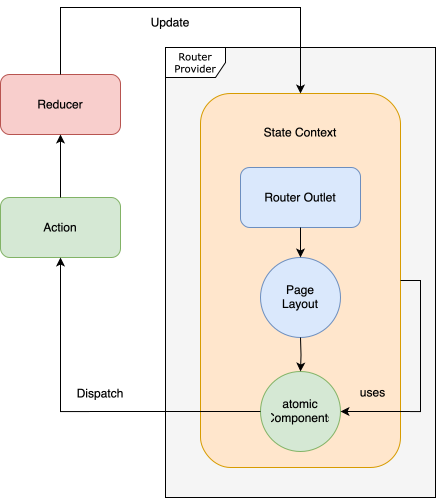
\includegraphics[width=\textwidth]{assets/Flow-Diagram.png}
  \label{fig:flow_chart}
\end{figure}

Pages (rectangles) and Components (circles) that are involved in updating and consuming the state context are presented in Figure  \ref{fig:uml_diagram}.

\begin{figure}[!h]
  \centering
  \caption{Flow of Components involved in updating and consuming the state context}
  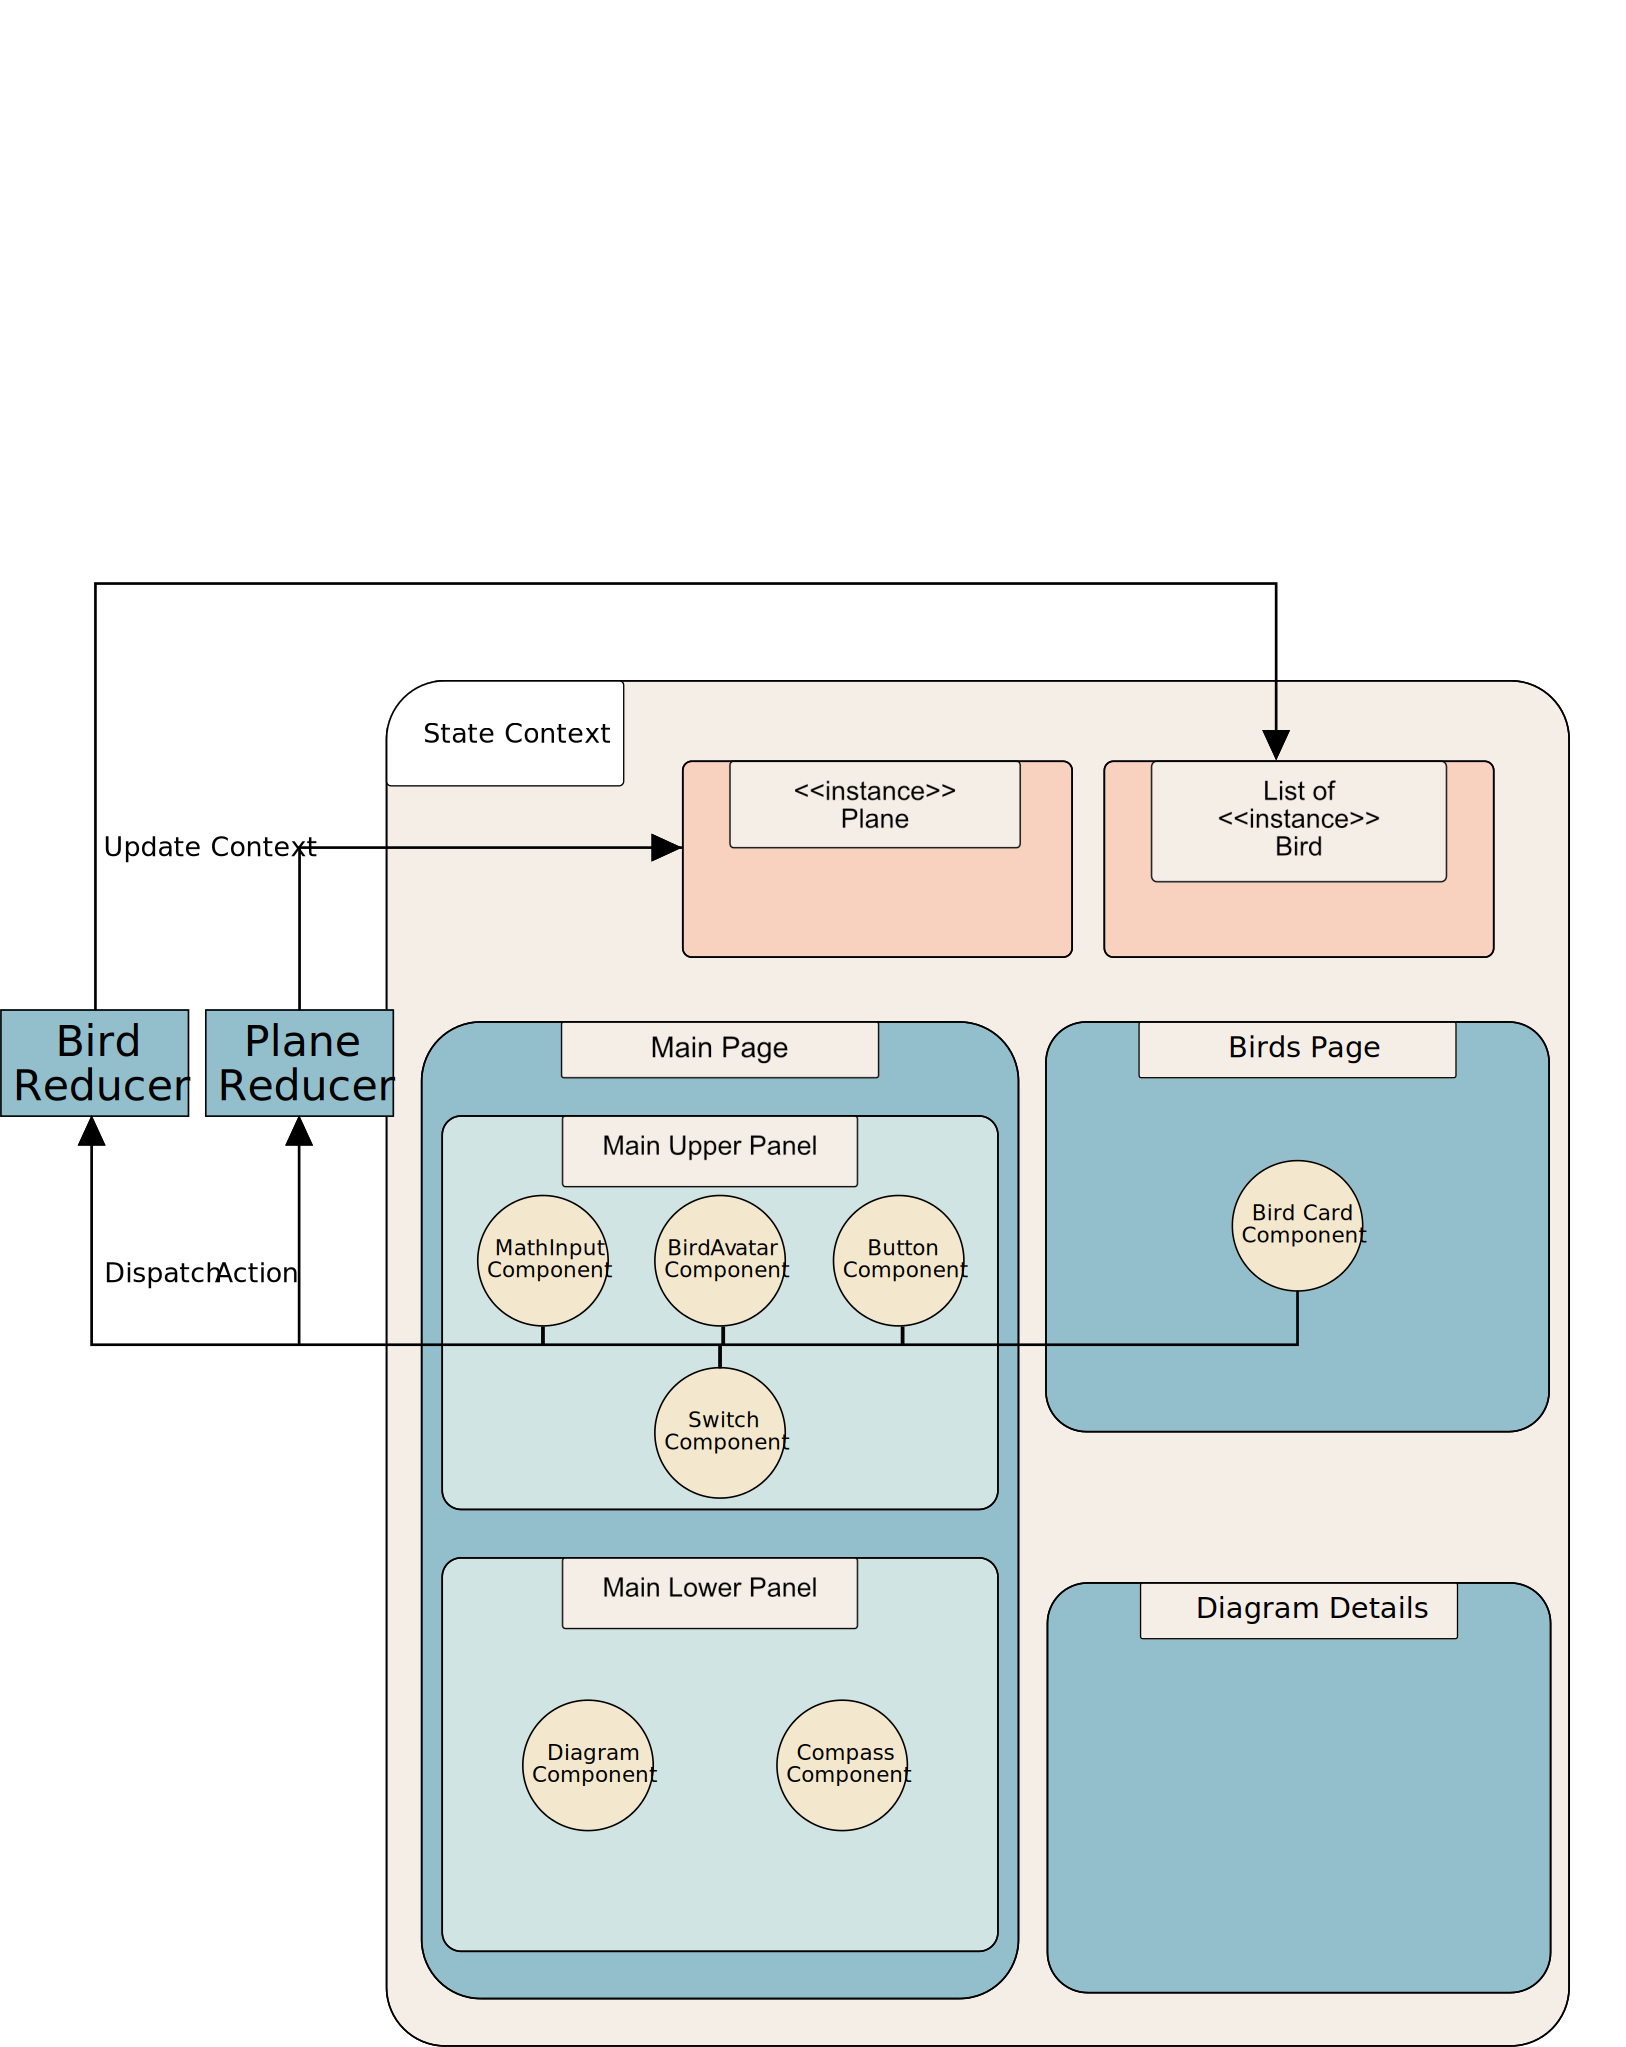
\includegraphics[width=\textwidth]{assets/uml_diagram.png}
  \label{fig:uml_diagram}
\end{figure}

\blankpage
\newpage
\subsection{Design and Implementation Procedure}
The design process was mostly defined by drawing and redefining new mock-ups that were refined after each sprint. The implementation of mathematical functions followed a \ac{TDD} procedure.

\subsection{Used 3rd Party Libraries}
The following 3rd party libraries were finally used in the making of this application.
\begin{itemize}
  \item React (\cite{React}), because of its simple design and vast ecosystem and the "ease" of state updates.
  \item React Router (\cite{ReactRouter}) as a well established way to navigate a website. 
  \item React Icons (\cite{ReactIcons}) as a nice and easy way to display common FontAwesome (\cite{FA}) Icons.
  \item Chakra-UI (\cite{chakra}), again for its ease of use and customizability of existing designs.
  \item PlotlyJS (\cite{PlotlyJS}), because it is the only graphing library I found that I could misuse for drawing shapes rather than the intended purpose of presenting data graphically. On top of it all it is well documented.
  \item Vite (\cite{Vite}) as a modern building tool, to get the app ready for production.
  \item Vitest (\cite{Vitest}), since I'm already using vite, the corresponding testing framework was the only logical choice.
  \item Docker (\cite{Docker}), which was not really necessary for my application in the end. But since the task asked for it, the webserver still runs as a dockerized container, running an NGINX \cite{NGINX} on the backend, serving the distribution version of this web application.
\end{itemize}